\subsection{Expected-loss decomposition}\label{sec:identification}

The holding leg carries two \emph{risks}, and they are what the expected loss prices. The baseline cost of converting under normal conditions is not a risk but a fee, the on- and off-ramp conversion basis; it belongs to the circuit of Section~\ref{sec:empirical_comparison} and is counted there once, not in the holding loss. The expected loss the holder bears for \emph{holding} the coin is therefore the counterparty exposure plus the stress depeg,
\[
  \Pi_{\text{risk}} = \underbrace{\ell_C}_{\text{counterparty},\ h\xi} + \underbrace{\ell_{D,s}}_{\text{stress, the game}},
\]
with the counterparty piece read from market proxies and the stress piece the endogenous stress probability of Proposition~\ref{prop:ps} times the depeg realised when primary redemption is exhausted.

At the parametrisation of Table~\ref{tab:cg_params}, USDC's holding loss is $\Pi_{\text{risk}}^{\text{USDC}} = 21$ basis points, 20 of counterparty risk and about 1 of probability-weighted stress depeg (the $0.0052$ endogenous stress probability times a stress depeg of the order of the SVB episode). USDT's is $\Pi_{\text{risk}}^{\text{USDT}} = 60$ basis points, 60 of counterparty risk and a negligible stress piece, since its primary redemption stayed open through the Terra fallout and its endogenous stress probability is $0.00031$. Table~\ref{tab:dual_asset_premium} reports the two side by side. The conversion fees that complete the cost of a payment, the on-ramp and off-ramp basis and platform charges, enter the corridor comparison of Section~\ref{sec:empirical_comparison}.

\begin{table}[H]
\centering
\caption{Holding-leg expected loss for the two stablecoins, in basis points. The loss is counterparty plus stress depeg; the baseline conversion cost is a circuit fee (Section~\ref{sec:empirical_comparison}), not a holding risk. The stress depeg is the closed-form model output.}\label{tab:dual_asset_premium}
\begin{tabular}{lrrl}
\toprule
Component & USDC & USDT & Source \\
\midrule
$\ell_C$ counterparty            & 20.0 (94\%) & 60.0 (100\%) & market proxies ($h,\xi$) \\
$\ell_{D,s}$ stress depeg         & \phantom{0}1.3 \phantom{00}(6\%)  & \phantom{00}0.0 \phantom{0}(0\%) & global game $\times\, p_s$ \\
$\Pi_{\text{risk}}$ holding loss  & 21.3        & 60.0        & both counterparty-led \\
\bottomrule
\end{tabular}
\end{table}

Once the conversion fee is recognised as a fee, both holding losses are counterparty-led, but the residual risk separates the two coins on a different axis. USDC carries a non-trivial stress depeg: its primary redemption is vulnerable to suspension, as the SVB weekend showed, so the secondary market does the work and the coordination run is priced. USDT carries almost none: its primary redemption stayed open through Terra, so the run never priced, and its loss is the counterparty exposure of an opaque reserve. The heterogeneity is therefore counterparty against stress depeg, not counterparty against a conversion cost. The level is dominated by the counterparty term; across the plausible range of the externally set $(h,\xi)$ the holding loss ranges over roughly $[16,37]$ basis points for USDC and $[49,99]$ for USDT (Appendix~\ref{app:sensitivity}), and the model's stress piece, small in expectation because the deep trough is a tail event, moves the total by about a basis point. We carry both holding losses, and the conversion fees that complete the circuit, into Section~\ref{sec:empirical_comparison}.

\subsection{Mechanism check: depeg and redemption flows}\label{sub:mechanism_check}

The calibration imposes the model's depeg channel; we now check that channel against the data directly. The model's secondary price falls in unmet redemption pressure, convexly and the more steeply the thinner the market (Proposition~\ref{prop:reserves} and the price-impact function~\eqref{eq:psec}). We proxy redemption pressure by the daily net outflow of circulating supply (mint and burn, from DefiLlama) and the realised depeg by the daily maximum below-par deviation of the hourly secondary price (CryptoCompare), and regress one on the other, by issuer, over 2022--2026 (Table~\ref{tab:mechanism_check}).

\begin{table}[H]
\centering
\caption{Mechanism check. Daily depeg (basis points) on daily net redemption outflow (percent of circulating supply), by issuer over 2022--2026, redemption days only; outflows from DefiLlama mint-burn data, prices from CryptoCompare; HC1 $t$-statistics in parentheses.}\label{tab:mechanism_check}
\begin{tabular}{lrr}
\toprule
 & USDC & USDT \\
\midrule
Outflow slope (bps per 1\% outflow) & 27.5 \;(1.6) & 15.1 \;(2.1) \\
Quadratic term in outflow           & $+28.8$ \;(2.0) & $-7.0$ \;($-2.2$) \\
Shape of response                    & convex & concave \\
$R^2$ (quadratic)                    & 0.18 & 0.17 \\
Redemption days                      & 790 & 482 \\
\bottomrule
\end{tabular}
\end{table}

The model's sharpest prediction is a threshold: with unmet redemption $U = \max(D-R,0)$, the depeg should stay near zero until net redemptions exceed liquid reserves and then rise convexly. For USDC the data show exactly this kink. Estimating a breakpoint by grid search, the depeg is flat until net redemptions reach about $1.1\%$ of circulating supply and then rises at roughly 90 basis points per additional percentage point, nearly doubling the fit of a linear specification ($R^2$ of 0.17 against 0.08). For USDT no threshold is detected ($\hat\gamma \approx 0$), consistent with a deeper market that absorbs redemptions across the observed range. The same depth gap shows in the curvature of the unrestricted fit (Table~\ref{tab:mechanism_check}): the depeg rises with net redemptions for both issuers (15 to 28 basis points per percentage point), convexly for the thin USDC market and roughly linearly for the deep USDT one, the cross-issuer pattern the calibrated depth gap of Section~\ref{sub:not_homogeneous} predicts, recovered from the data without using the model.\footnote{The regression documents the conditional shape the model predicts rather than a causal slope: depeg and outflow are jointly determined within a run, and the largest observed outflow (3.6\% of supply) only borders the region where redemptions exceed liquid reserves, which is why it serves as a mechanism check rather than as an estimation input.}

These two episodes are plotted in Section~\ref{sec:risk_factors} (Figures~\ref{fig:svb_onchain} and~\ref{fig:terra_onchain}); the regression here is their quantitative counterpart. The realised depeg is severe when primary redemption is suspended, as for USDC over the SVB weekend, and mild when it is honoured at par, as for USDT over the Terra fallout.

\subsection{Mapping heterogeneity across the stablecoin universe}\label{sub:cross_section}

The two coins we calibrate, USDC and USDT, are the two largest fiat-backed stablecoins, together over 90\% of the segment. The rest of the universe varies along the two primitives the model identifies, reserve composition and secondary market depth. Table~\ref{tab:cross_section} maps that variation: the realised depeg of seven fiat-backed stablecoins in the two systemic episodes, measured as the trough of the hourly secondary price.

\begin{table}[H]
\centering
\caption{Realised depeg of fiat-backed stablecoins in the two systemic episodes (trough of the hourly secondary price, basis points below par; CryptoCompare), ordered by the March 2023 depeg. The fractional-algorithmic FRAX is excluded as outside the fiat-backed scope.}\label{tab:cross_section}
\begin{tabular}{llrr}
\toprule
Stablecoin & Reserve profile & SVB 2023 & Terra 2022 \\
\midrule
DAI  & Crypto-collateralised, then majority USDC & 1082 & 24 \\
USDC & Treasuries and cash, exposed to SVB        & 978  & 16 \\
USDP & Treasuries and cash (Paxos), thin market   & 914  & 122 \\
GUSD & Treasuries and cash (Gemini), thin market  & 494  & 285 \\
TUSD & Mixed reserves, attestation-only           & 345  & 168 \\
BUSD & Treasuries (Paxos), segregated             & 17   & 36 \\
USDT & Mixed, offshore, attestation-only          & 4    & 249 \\
\bottomrule
\end{tabular}
\end{table}

The cross-section reproduces the reserve-quality comparative static of Proposition~\ref{prop:reserves} across issuers, and it does so with the sign reversing between episodes. In the March 2023 banking episode the depeg tracked exposure to the failed US bank: USDC, which held part of its cash reserve at Silicon Valley Bank, fell to 0.90, and DAI, then majority-collateralised by USDC, to 0.89, while the offshore USDT and the segregated-reserve BUSD held within twenty basis points of par; the smaller USDP, GUSD, and TUSD depegged by intermediate amounts, amplified by their thinner secondary markets. In the May 2022 Terra contagion the ordering inverts: the mixed-reserve, offshore USDT fell to 0.975 and the thin Gemini dollar to 0.97, while the clean, deep USDC barely moved. The two coins we calibrate therefore sit at opposite ends in opposite episodes, which is the inverted-composition result of Section~\ref{sec:identification} seen across the segment: a stablecoin's vulnerability is set by its reserve composition and secondary market depth relative to the shock, not by the category label. USDC and USDT are the two poles of this map, and the calibrated expected losses bracket the range the segment spans. Figure~\ref{fig:cross_section_map} plots the seven coins on the plane of the two episodes: USDC and USDT occupy opposite corners, while the remaining coins scatter between them according to their exposure to each shock, GUSD vulnerable to both and the segregated-reserve BUSD to neither.

\begin{figure}[H]
\centering
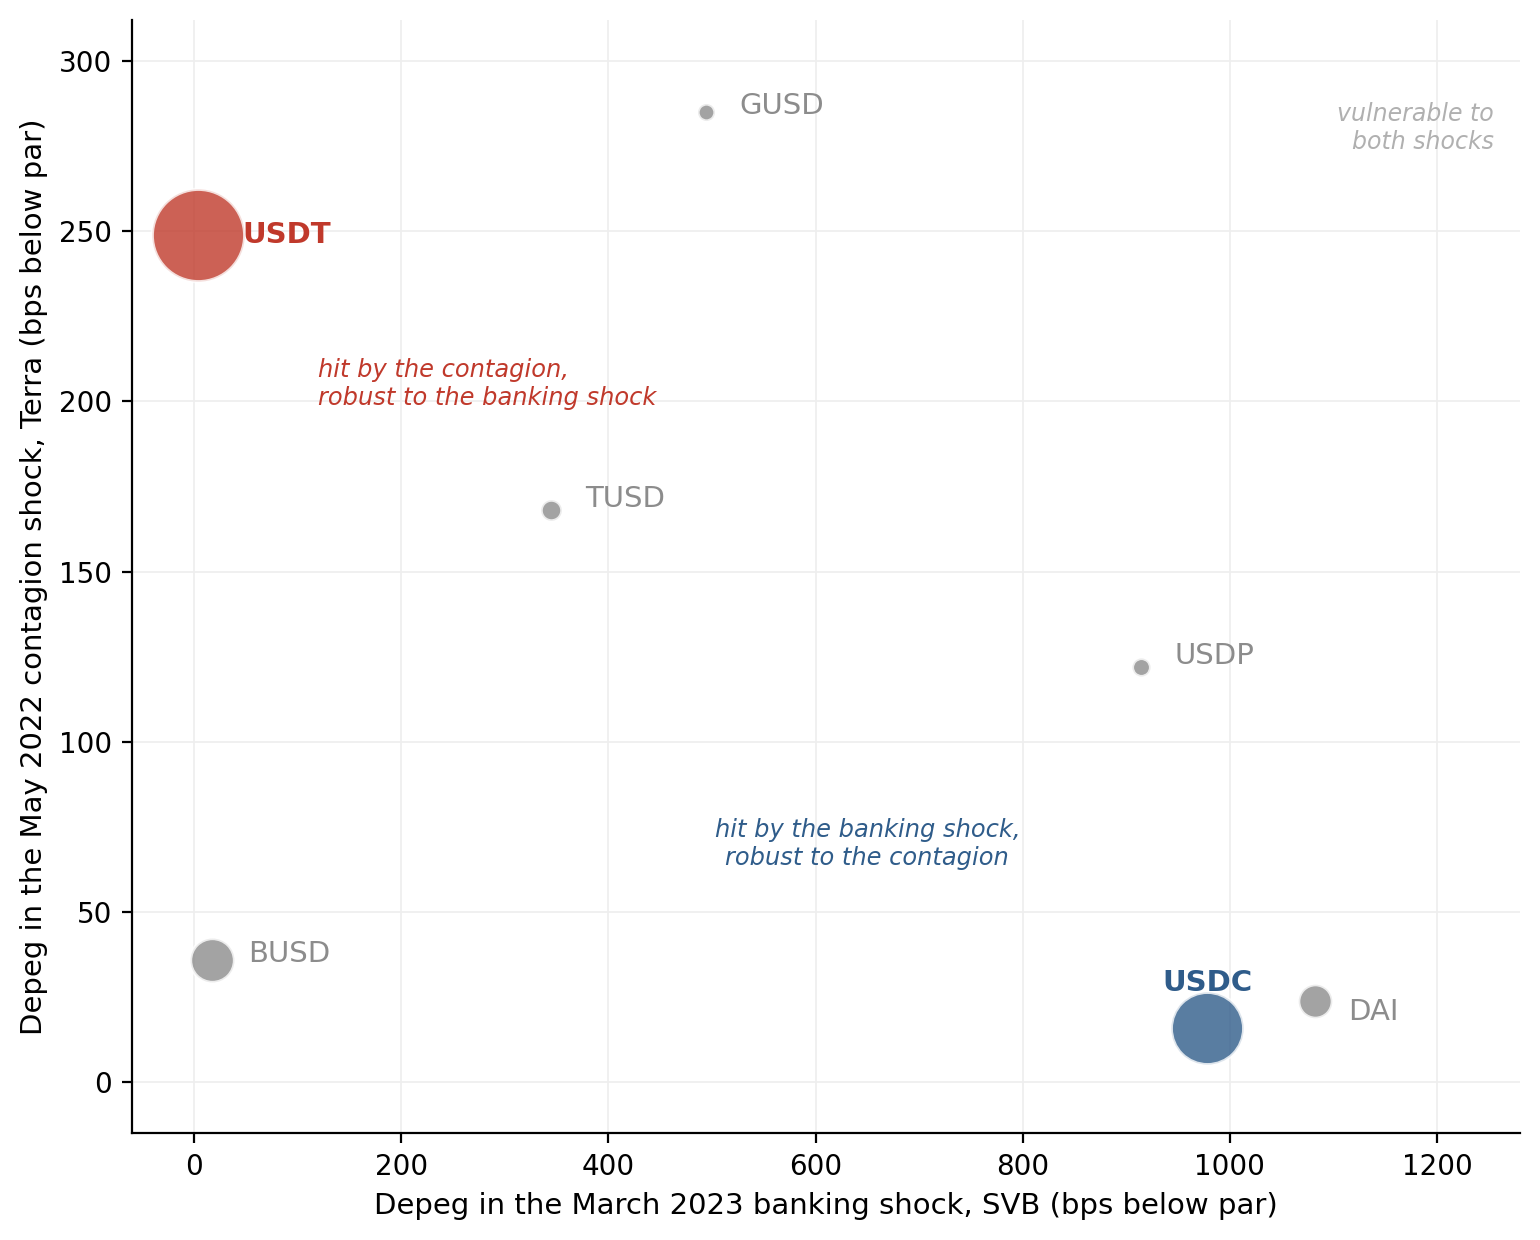
\includegraphics[width=0.92\textwidth]{figures/fig_cross_section_map.pdf}
\caption{Realised depeg of seven fiat-backed stablecoins in the two systemic episodes (trough of the hourly secondary price, basis points below par; CryptoCompare), plotted as the March 2023 banking-shock depeg against the May 2022 contagion-shock depeg. Bubble area is the coin's approximate peak circulating supply over 2022--2023, and USDC and USDT are highlighted as the two calibrated coins. A coin's vulnerability is shock-specific: USDC and DAI fall hard in the banking shock but not the contagion, USDT the reverse, so the two calibrated coins sit in opposite corners. Computed from realised prices alone, independently of the model.}\label{fig:cross_section_map}
\end{figure}
